% 使用 xelatex 编译
\documentclass[UTF8,a4paper,twoside,zihao=-4]{ctexrep}
%%%% 文档类设置 %%%%%%%%
\ctexset{
	contentsname = {目\quad 录},
	chapter = {
		beforeskip = 0pt,
		afterskip = 20pt,
		name = {第,章},
		nameformat = \zihao{3}\bfseries,
		number = \Chinese{chapter},
		numberformat = \zihao{3}\bfseries,
		titleformat = \zihao{3}\bfseries,
		fixskip = true,
		%afterindent = false
		        },
	section = {
		beforeskip = \ccwd,
		afterskip =1ex plus 0.2ex,
		format = \raggedright,
		nameformat = \zihao{4}\bfseries,
		numberformat = \zihao{4}\bfseries,
		titleformat = \zihao{4}\bfseries,
		%afterindent = false
			},
	subsection = {
		beforeskip =\ccwd,
		afterskip = 0.5ex plus 0.1ex,
		format = \raggedright,
		nameformat = \zihao{-4}\bfseries,
		numberformat = \zihao{-4}\bfseries,
		titleformat = \zihao{-4}\bfseries
			}
	    }

%%%% 宏包 %%%%%%%%%%%
\usepackage{amsmath,amssymb,amsfonts}
\usepackage{graphicx}
\usepackage{ulem}
\usepackage{pdfpages}
\usepackage{lipsum}
%%%% 页面设置 %%%%%%%%%%%%%%%%%%%%%%
\usepackage[bindingoffset=.5cm,centering,includeheadfoot,margin=2.5cm]{geometry}
\setlength\parskip{0pt}
\usepackage{fancyhdr}
	\pagestyle{fancy}
	\fancyhead[LE,RO]{\thepage}
	\fancyhead[RE]{\textsl{\nouppercase{\leftmark}}}
	\fancyhead[LO]{\textsl{\nouppercase{\rightmark}}}
	\fancyfoot{}
	%\renewcommand{\headrulewidth}{0pt}
\renewcommand\sectionmark[1]{%
	\markright{\CTEXifname{\CTEXthesection\quad}{}#1}}
\usepackage[colorlinks,linkcolor=blue,bookmarks=true]{hyperref}
%%%% 字体 %%%%%%%%%
\usepackage{lmodern}
\setCJKmainfont[
	BoldFont=AdobeHeitiStd-Regular.otf,
	ItalicFont=AdobeKaitiStd-Regular.otf
				]{simsun.ttc}
%%%%%%%%%%%%%%%%%%%%%%
%%%%%%%%%%%%%%%%%%%%%%
%%%%%%%%%%%%%%%%%%%%%%
\begin{document}
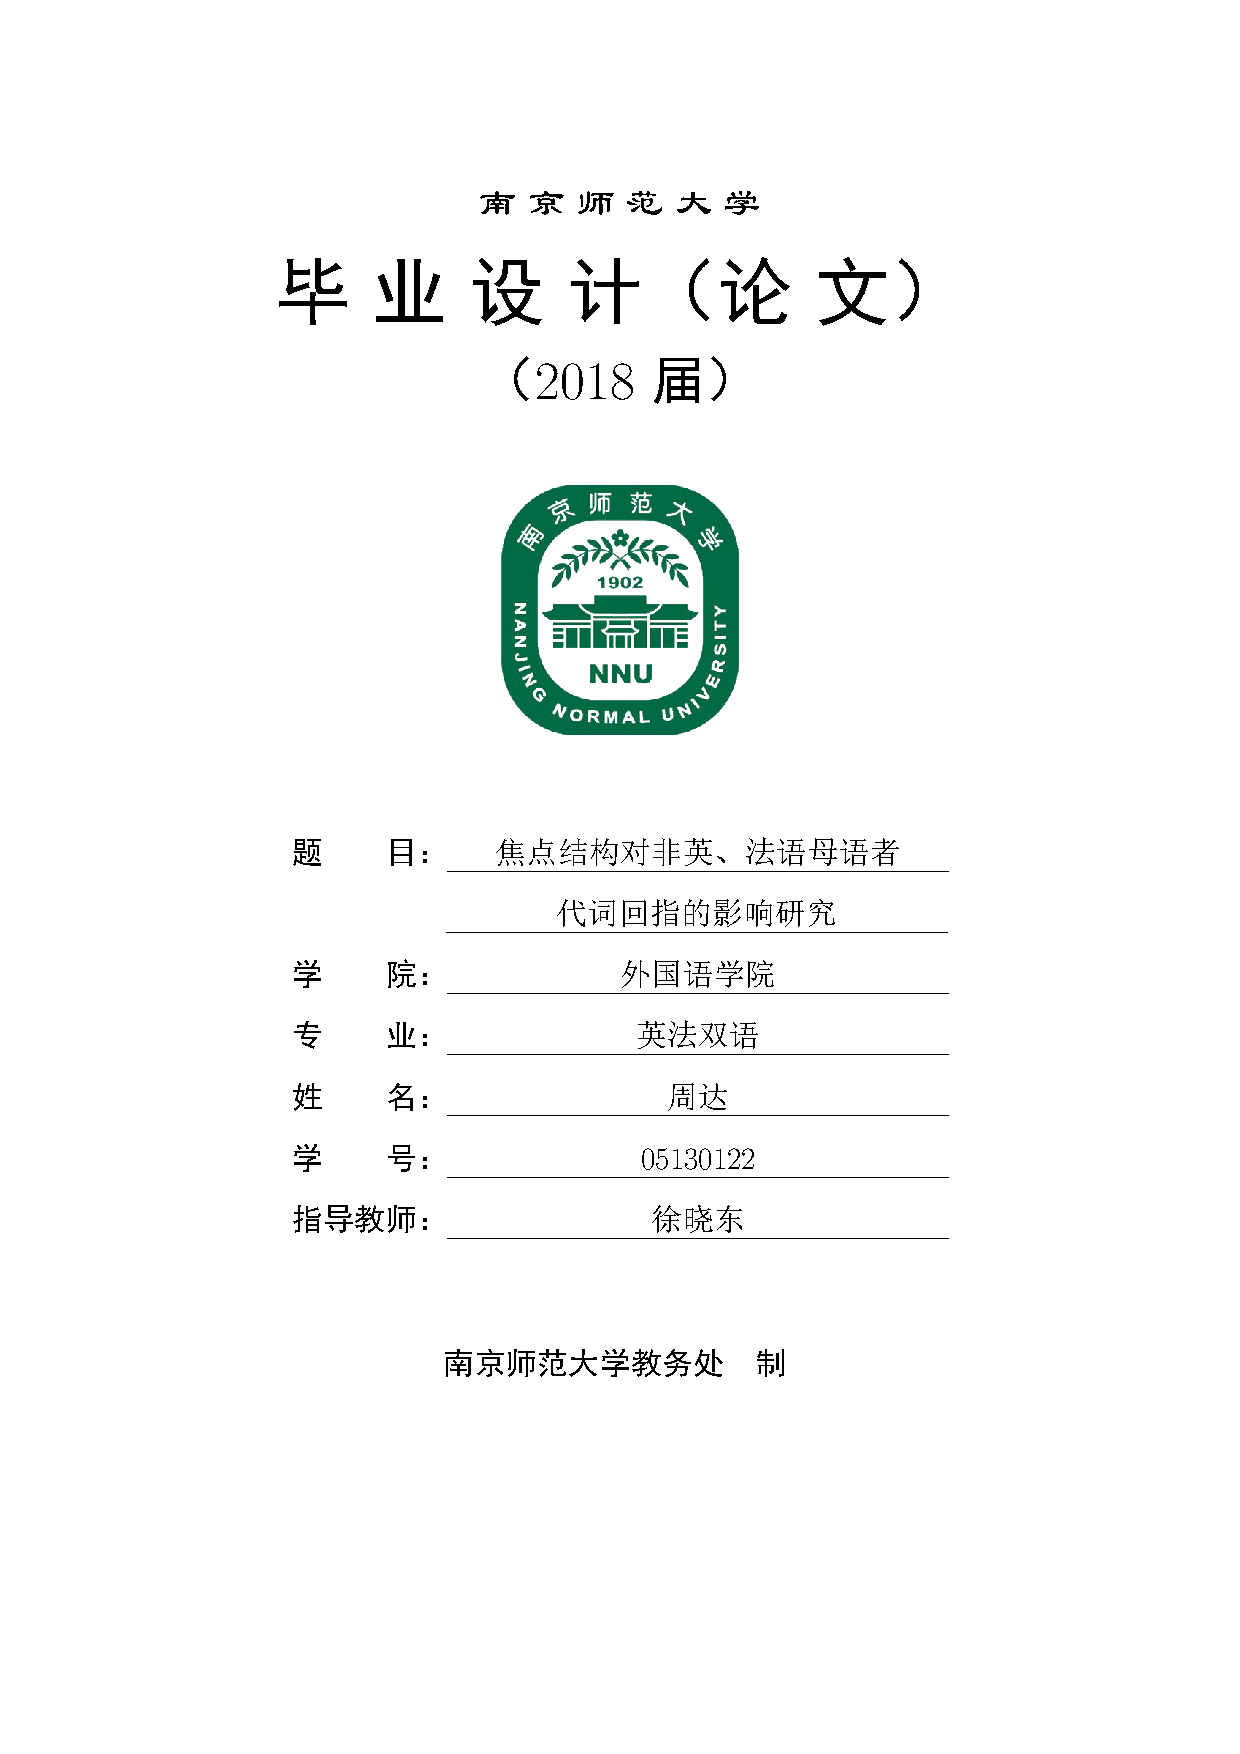
\includepdf{cover/cover.pdf} %%%%% 封面 %%%%%%%%%%%%
%%%%%%% 中英文摘要 %%%%%%%%%%%%%%%%
%%% 中文摘要
\clearpage
\thispagestyle{plain}
\phantomsection
\addcontentsline{toc}{chapter}{摘\quad 要}

\centerline{\zihao{3}\heiti 摘\quad 要}

\linespread{1.4}\zihao{-4} \bigskip

本文探讨了英语和法语非母语者的语言处理过程中,焦点结构和代词回指之间的关系。首先我们从语法和语用角度,梳理了关于焦点作用和代词回指机制的研究现状。接着通过设计自定步速阅读实验,我们发现以分裂句为形式的焦点结构不一定能提升语言片段的显著性,并使其更可能成为代词回指的对象,这与前人的研究结果是相符的。在我们的测试中,法语主语位置的焦点和英语宾语位置的焦点反应时间都较短,但两种语言的主语焦点都导致了更长的回指反应时间。另外,我们还发现焦点和回指对象的一致性并不能提升焦点位置的显著性。因此本文认为,英语和法语中是否存在主语或宾语回指偏向的问题,比当前已有研究结论更加复杂。
\bigskip

\noindent{\zihao{4}\heiti 关键词:}
焦点作用, 代词回指, 自定步速阅读, 英语, 法语

% Abstract
\clearpage
\thispagestyle{plain}
\phantomsection
\addcontentsline{toc}{chapter}{Abstract}

\centerline{\zihao{3}\bfseries Abstract}

\linespread{1.4}\zihao{-4}
\bigskip

This thesis explores the relationship between focus structure and pronoun resolution among non-native speakers of English and French. Firstly we reviewed the existing literature on the mechanism of focus effect and pronoun resolution. Then through a self-paced reading test, we find that focus, in the form of cleft structure does not necessarily increase the salience of a informational unit, thus may not in some cases make it a preferred antecedent for pronoun resolution. This result is line with previous researches on this topic. In our experiment, We also find that focused subject in French and focused object in English are processed faster, but focused subjects in both languages leads to longer response time of anaphora. Furthermore, our research also shows that the congruence between anaphora and focus does not make the latter more accessible. In this regard, we argue that the problem of whether there is subject or object preference in English and French is more complicated than the results of current studies.

\bigskip
\noindent\textbf{\zihao{4} Keywords:} 
focus effect, pronoun resolution, self-paced reading, English, French


\tableofcontents\newpage\mbox{}\thispagestyle{empty}\newpage
\clearpage\pagenumbering{arabic}
\chapter{绪论}
来一回《三国演义》
\section{宴桃园豪杰三结义\quad 斩黄巾英雄首立功}
话说天下大势,分久必合,合久必分。周末七国分争,并入于秦。及秦灭之后,楚、汉分争,又并入于汉。汉朝自高祖斩白蛇而起义,一统天下,后来光武中兴,传至献帝,遂分为三国。推其致乱之由,殆始于桓、灵二帝。桓帝禁锢善类,崇信宦官。及
桓帝崩,灵帝即位,大将军窦武、太傅陈蕃共相辅佐。时有宦官曹节等弄权,窦武、陈蕃谋诛之,机事不密,反为所害,中涓自此愈横\footnote{这是一个脚注。}。

建宁二年四月望日,帝御温德殿。方升座,殿角狂风骤起。只见一条大青蛇,从梁上飞将下来,蟠于椅上。帝惊倒,左右急救入宫,百官俱奔避。须臾,蛇不见了。忽然大雷大雨,加以冰雹,落到半夜方止,坏却房屋无数。建宁四年二月,洛阳地震;又海水泛溢,沿海居民,尽被大浪卷入海中。光和元年,雌鸡化雄。六月朔,黑气十余丈,飞入温德殿中。秋七月,有虹现于玉堂;五原山岸,尽皆崩裂。种种不祥,非止一端。帝下诏问群臣以灾异之由,议郎蔡邕上疏,以为蜺堕鸡化,乃妇寺干政之所致,言颇切直。帝览奏叹息,因起更衣。曹节在后窃视,悉宣告左右;遂以他事陷邕于罪,放归田里。后张让、赵忠、封谞、段珪、曹节、侯览、蹇硕、程旷、夏恽、郭胜十人朋比为奸,号为``十常侍''。帝尊信张让,呼为``阿父''。朝政日非,以致天下人心思乱,盗贼蜂起。
\subsection{加一级标题}

时巨鹿郡有兄弟三人,一名张角,一名张宝,一名张梁。那张角本是个不第秀才,因入山采药,遇一老人,碧眼童颜,手执藜杖,唤角至一洞中,以天书三卷授之,曰:``此名《太平要术》,汝得之,当代天宣化,普救世人;若萌异心,必获恶报。''角拜问姓名。老人曰:``吾乃南华老仙也。''言讫,化阵清风而去。角得此书,晓夜攻习,能呼风唤雨,号为``太平道人"。中平元年正月内,疫气流行,张角散施符水,为人治病,自称``大贤良师"。角有徒弟五百余人,云游四方,皆能书符念咒。次后徒众日多,角乃立三十六方,大方万余人,小方六七千,各立渠帅,称为将军;讹言:``苍天已死,黄天当立;岁在甲子,天下大吉。"令人各以白土书``甲子"二字于家中大门上。青、幽、徐、冀、荆、扬、兖、豫八州之人,家家侍奉大贤良师张角名字。角遣其党马元义,暗赍金帛,结交中涓封谞,以为内应。角与二弟商议曰:``至难得者,民心也。今民心已顺,若不乘势取天下,诚为可惜。"遂一面私造黄旗,约期举事;一面使弟子唐周,驰书报封谞。唐周乃径赴省中告变。帝召大将军何进调兵擒马元义,斩之;次收封谞等一干人下狱。张角闻知事露,星夜举兵,自称``天公将军",张宝称``地公将军",张梁称``人公将军"。申言于众曰:``今汉运将终,大圣人出。汝等皆宜顺天从正,以乐太平。''四方百姓,裹黄巾从张角反者四五十万。贼势浩大,官军望风而靡。何进奏帝火速降诏,令各处备御,讨贼立功。一面遣中郎将卢植、皇甫嵩、朱儁,各引精兵、分三路讨之。

且说张角一军,前犯幽州界分。幽州太守刘焉,乃江夏竟陵人氏,汉鲁恭王之后也。当时闻得贼兵将至,召校尉邹靖计议。靖曰:``贼兵众,我兵寡,明公宜作速招军应敌。''刘焉然其说,随即出榜招募义兵。

榜文行到涿县,引出涿县中一个英雄。那人不甚好读书;性宽和,寡言语,喜怒不形于色;素有大志,专好结交天下豪杰;生得身长七尺五寸,两耳垂肩,双手过膝,目能自顾其耳,面如冠玉,唇若涂脂;中山靖王刘胜之后,汉景帝阁下玄孙,姓刘名备,字玄德。昔刘胜之子刘贞,汉武时封涿鹿亭侯,后坐酎金失侯,因此遗这一枝在涿县。玄德祖刘雄,父刘弘。弘曾举孝廉,亦尝作吏,早丧。玄德幼孤,事母至孝;家贫,贩屦织席为业。家住本县楼桑村。其家之东南,有一大桑树,高五丈余,遥望之,童童如车盖。相者云:"此家必出贵人。"玄德幼时,与乡中小儿戏于树下,曰:``我为天子,当乘此车盖。"叔父刘元起奇其言,曰:``此儿非常人也!"因见玄德家贫,常资给之。年十五岁,母使游学,尝师事郑玄、卢植,与公孙瓒等为友。

及刘焉发榜招军时,玄德年已二十八岁矣。当日见了榜文,慨然长叹。随后一人厉声言曰:``大丈夫不与国家出力,何故长叹?"玄德回视其人,身长八尺,豹头环眼,燕颔虎须,声若巨雷,势如奔马。玄德见他形貌异常,问其姓名。其人曰:``某姓张名飞,字翼德。世居涿郡,颇有庄田,卖酒屠猪,专好结交天下豪杰。恰才见公看榜而叹,故此相问。"玄德曰:``我本汉室宗亲,姓刘,名备。今闻黄巾倡乱,有志欲破贼安民,恨力不能,故长叹耳。"飞曰:``吾颇有资财,当招募乡勇,与公同举大事,如何。"玄德甚喜,遂与同入村店中饮酒。

正饮间,见一大汉,推着一辆车子,到店门首歇了,入店坐下,便唤酒保:``快斟酒来吃,我待赶入城去投军。"玄德看其人:身长九尺,髯长二尺;面如重枣,唇若涂脂;丹凤眼,卧蚕眉,相貌堂堂,威风凛凛。玄德就邀他同坐,叩其姓名。其人曰:``吾姓关名羽,字长生,后改云长,河东解良人也。因本处势豪倚势凌人,被吾杀了,逃难江湖,五六年矣。今闻此处招军破贼,特来应募。"玄德遂以己志告之,云长大喜。同到张飞庄上,共议大事。飞曰:``吾庄后有一桃园,花开正盛;明日当于园中祭告天地,我三人结为兄弟,协力同心,然后可图大事。"玄德、云长齐声应曰:``如此甚好。"

次日,于桃园中,备下乌牛白马祭礼等项,三人焚香再拜而说誓曰:``念刘备、关羽、张飞,虽然异姓,既结为兄弟,则同心协力,救困扶危;上报国家,下安黎庶。不求同年同月同日生,只愿同年同月同日死。皇天后土,实鉴此心,背义忘恩,天人共戮!"誓毕,拜玄德为兄,关羽次之,张飞为弟。祭罢天地,复宰牛设酒,聚乡中勇士,得三百余人,就桃园中痛饮一醉。来日收拾军器,但恨无马匹可乘。正思虑间,人报有两个客人,引一伙伴当,赶一群马,投庄上来。玄德曰:``此天佑我也!"三人出庄迎接。原来二客乃中山大商:一名张世平,一名苏双,每年往北贩马,近因寇发而回。玄德请二人到庄,置酒管待,诉说欲讨贼安民之意。二客大喜,愿将良马五十匹相送;又赠金银五百两,镔铁一千斤,以资器用。

\chapter{Typing English}
Just some nonsense\dots
\section{Beautiful Fonts}
\lipsum
\chapter{\LaTeX\ \&\ Mathematics}
\section{Euler Constant}
\[
\begin{aligned}
	\gamma&=\lim_{n\to\infty}\left(-\ln n+\sum_{k=1}^{n}\frac{1}{k}\right)\\
		   &=\int^{\infty}_{1}\left(\frac{1}{\lfloor x\rfloor}-\frac{1}{x}\right) dx
\end{aligned}
\]
\chapter{结语}
\begin{thebibliography}{99}
\addcontentsline{toc}{chapter}{参考文献}
\bibitem{LiuLaTeX}
	刘海洋, 《\LaTeX 入门》, 电子工业出版社, 2013.
\bibitem{GGMM}
	George Gr\"{a}tzer, \emph{More Math Into \LaTeX}, Springer, 2016.
\end{thebibliography}
\end{document}